%%%%%%%%%%%%%%%%%%%%%%%%%%%%%
% Standard header for working papers
%
% WPHeader.tex
%
%%%%%%%%%%%%%%%%%%%%%%%%%%%%%

\documentclass[11pt]{article}

%%%%%%%%%%%%%%%%%%%%
%% Include general header where common packages are defined
%%%%%%%%%%%%%%%%%%%%



%%%%%%%%%%%%%%%%%%%%%%%%%%
%% Packages
%%%%%%%%%%%%%%%%%%%%%%%%%%


% general packages without options
\usepackage{amsmath,amssymb,bbm}

% graphics
\usepackage{graphicx}

% text formatting
\usepackage[document]{ragged2e}
\usepackage{pagecolor,color}




\usepackage[utf8]{inputenc}
\usepackage[T1]{fontenc}
%\usepackage[francais]{babel}



% for framed figures or texts
\usepackage{mdframed}



%%%%%%%%%%%%%%%%%%%%
%% Idem general commands
%%%%%%%%%%%%%%%%%%%%
%% Commands

\newcommand{\noun}[1]{\textsc{#1}}


%% Math

% Operators
\DeclareMathOperator{\Cov}{Cov}
\DeclareMathOperator{\Var}{Var}
\DeclareMathOperator{\E}{\mathbb{E}}
\DeclareMathOperator{\Proba}{\mathbb{P}}

\newcommand{\Covb}[2]{\ensuremath{\Cov\!\left[#1,#2\right]}}
\newcommand{\Eb}[1]{\ensuremath{\E\!\left[#1\right]}}
\newcommand{\Pb}[1]{\ensuremath{\Proba\!\left[#1\right]}}
\newcommand{\Varb}[1]{\ensuremath{\Var\!\left[#1\right]}}

% norm
\newcommand{\norm}[1]{\| #1 \|}


%% graphics

% renew graphics command for relative path providment only ?
%\renewcommand{\includegraphics[]{}}



% geometry
\usepackage[margin=2cm]{geometry}

\usepackage{float}

% layout : use fancyhdr package
\usepackage{fancyhdr}
\pagestyle{fancy}

\makeatletter

\renewcommand{\headrulewidth}{0.4pt}
\renewcommand{\footrulewidth}{0.4pt}
\fancyhead[RO,RE]{05/2017}
\fancyhead[LO,LE]{Examen Final}
\fancyfoot[RO,RE] {\thepage}
\fancyfoot[LO,LE] {L2 54EEG3GO - S4 2017}
\fancyfoot[CO,CE] {}


\fancypagestyle{firststyle}
{
   \fancyhf{}
   \fancyhead[RO,RE]{Examen Final - 05/2017}
   \fancyhead[LO,LE]{L2 54EEG3GO - S4 2017}
}


%\renewcommand{\abstractname}{Objectifs du TD}

\renewcommand{\figurename}{\textbf{Document}}

\newcommand{\question}[1]{$\rightarrow$ \textit{#1}}


\makeatother


%%%%%%%%%%%%%%%%%%%%%
%% Begin doc
%%%%%%%%%%%%%%%%%%%%%

\begin{document}









\title{\textbf{Analyse Spatiale - Examen Final}}

\date{}


\maketitle

\justify

\thispagestyle{firststyle}



\section*{Exercice : Mesures de Réseau et Résilience}

La description complète d'un réseau suppose la donnée d'une grande quantité d'information, puisque la moitié de la matrice d'adjacence est nécessaire dans le cas non-dirigé (matrice complète dans le cas dirigé). L'établissement de typologies, c'est à dire de sortes de classes d'équivalence topologiques au sens large, est une façon de voir les enjeux de la recherche actuelle sur les réseaux : existe-t-il des formes typiques de réseau, et comment les représenter dans une dimension réduite ? Relativement importante est la dimension épistémologique de cette interrogation fondamentale, qui peut sous certaines hypothèses être ramenée à l'opposition d'un réductionisme à une vision intrinsèque de la complexité. Si une classification systématique réductrice existe pour tout système complexe, alors les niveaux d'émergence supérieurs n'ont pas de signification propre. Il est paradoxal d'observer dans ce cas la position ambigüe de certains travaux de physiciens qui tiennent ce réductionisme comme un dogmatisme mais prétendent s'attaquer à des problèmes complexes typiques des systèmes socio-techniques.

Les mesures de réseau globales comme nous avons vu en cours sont une façon de répondre partiellement à cette question de réduction dimensionnelle. En pratique, on veut être également capable de relier ces mesures à des propriétés pratiques du réseau, qui seront cruciales pour le design et le management de réseaux réels (par exemple réseaux techniques : transport d'électricité, internet ; réseaux de transport ; réseaux sociaux ; réseaux de villes ; etc.) : par exemple le coût, la résilience, la performance. Cet exercice propose de survoler ces deux questions fondamentales pour différents exemples de réseaux réels et synthétiques : illustrer dans un premier temps la signification concrète de différentes valeurs en relation à la topologie ``apparente'' du réseau ; dans un second temps explorer des liens potentiels entre mesures et propriétés afin de donner une idée d'une manière de caractériser la résilience.

Ce qui est demandé pourra paraître relativement simple mais est central pour une appréhension juste de la complexité des processus géographiques tels qu'ils occurrent dans toute leur réalité. La table~\ref{tab:measures} donne les valeurs d'indicateurs, pour certains types de réseaux. On fournit leur valeur moyenne et leur écart-type dans le cas de réseaux synthétiques aléatoires pour lesquels les mesures auront alors été estimées sur $N=1000$ répétitions des réseaux aléatoires.\footnote{qu'on fixe comme arbitraire. Le problème du nombre de répétitions nécessaires pour une convergence raisonnable des indicateurs statistiques et hors du champ de ce devoir, et d'ailleurs un problème ouvert pour la plupart des modèles de simulation complexes puisque qu'on sait établir des intervalles de confiances soit sous certaines hypothèses théoriques de distribution statistique soit par simulation (\emph{bootstrap}) ce qui ne réduit pas la complexité intrinsèque.} Pour les réseaux réels ou synthétiques non variables, une valeur seule est donnée, sachant que l'estimation de paramètres moyens dans des situations réelles est directement liée à la stationnarité spatio-temporelle des processus\footnote{et donc à leur ergodicité, i.e. à l'équivalence entre moyenne spatiale et moyenne temporelle}, ce qui est également une question ouverte concernant les systèmes spatiaux complexes. Les figures~\ref{fig:examples} et ~\ref{fig:real} illustre des exemples des réseaux considérés. Les questions suivantes portent sur une interprétation simple des mesures. Parmi les réseaux considérés, on étudie des réseaux routiers réels, dont la localisation spatiales est présentée en figure~\ref{fig:loc}, ainsi que des réseaux synthétiques.

Les réseaux étudiés sont donc les suivants\footnote{chaque générateur synthétique a des paramètres propres, pour lesquels nous choisissons les valeurs par défaut suivantes : probabilité aléatoire d'Erdos-Renyi $p=0.005$ ; proportion de liens de la grille conservés $65\%$ ; attachement préférentiel : nouveau liens $m=10$, exposant $\alpha=1$, exposant de vieillissement $\beta = -2$, pas de vieillissement 100 ; nombre de feuille par branche de l'arbre $f=3$.} : 
\begin{itemize}
\item Réseau routiers réels (simplifiés à une résolution de 100m) : Paris, Ile-de-France, La Courtine (Creuse), Grand Lyon, London Metropolitan Area, Randstad
\item Aléatoire (probabilité fixe d'établir un lien entre chaque paire de noeud)
\item Attachement préférentiel (type Barabasi-Albert : les liens sont établis itérativement avec une probabilité proportionnelle au degré des noeuds)
\item Grille perturbée (grille régulière dont on retire une proportion fixée de liens)
\item Arbre (au nombre de feuilles par branche fixe)
\end{itemize}

Les mesures calculées pour un réseau $N=(V,E)$ sont :

\begin{itemize}
\item Statistiques descriptives : nombre de noeuds $\left|V\right|$ et nombre de liens $\left|E\right|$
\item Densité $\gamma$
\item Degré moyen $\bar{d}$
\item Diamètre\footnote{pour toutes les mesures liées au plus courts chemins, les distances topologiques et non pondérées ont été prises en compte, afin de permettre la comparabilité des réseaux réels et des réseaux synthétiques. Pour une comparabilité des réseaux réels ayant des couvertures géographiques d'étendue significativement différentes, il faut normaliser par le diamètre.} $\delta$
\item Centralité d'intermédiarité $b$ : s'agissant d'une mesure locale (associée ici aux liens), on considère sa moyenne $<b>$ et son niveau de hiérarchie\footnote{donné par la pente de la regression linéaire d'un fit brutal d'une loi rang-taille : $\log{b_i} = \beta + \alpha\cdot \log i$ où les $b_i$ sont triés par ordre decroissants.} $\alpha\left[b\right]$
\item Centralité de proximité $c$ : de même on calcule $<c>$ et $\alpha\left[c\right]$
\item Efficacité $e = \frac{2}{n\cdot (n-1)} \sum_{i<j} \frac{1}{d_{ij}}$ avec $d_{ij}$ distance topologique entre $i$ et $j$
\item Coefficient de clustering $t$, qui donne la probabilité que les voisins d'un noeud soient connectés
\item Modularité $\mu$ qui donne une mesure plus générale de la structure en communauté du graphe
\end{itemize}


\bigskip

\question{}







%%%%%%%%%%%%%%
\begin{table}
\begin{tabular}{c|c|c|c|c|c|c|c|c|c|c|c|}
\hline
Réseau & $\left|V\right|$ & $\left|E\right|$ & $\gamma$ & $\bar{d}$ & $\delta$ & $<b>$ & $\alpha \left[b\right]$ & $<c>$ & $\alpha\left[c\right]$ & $e$ & $t$ & $\mu$\\\hline
Aléatoire & $\left|V\right|$ & $\left|E\right|$ & $\gamma$ & $d$ & $<b>$ & $\alpha \left[b\right]$ & $<c>$ & $\alpha\left[c\right]$ & $e$ & $t$ & $\mu$\\\hline
\end{tabular}
\caption{Valeurs de mesures de réseaux pour différents exemples typiques réels et synthétiques \label{tab:measures}}
\end{table}
%%%%%%%%%%%%%%


%%%%%%%%%%%%%%
\begin{figure}
\centering
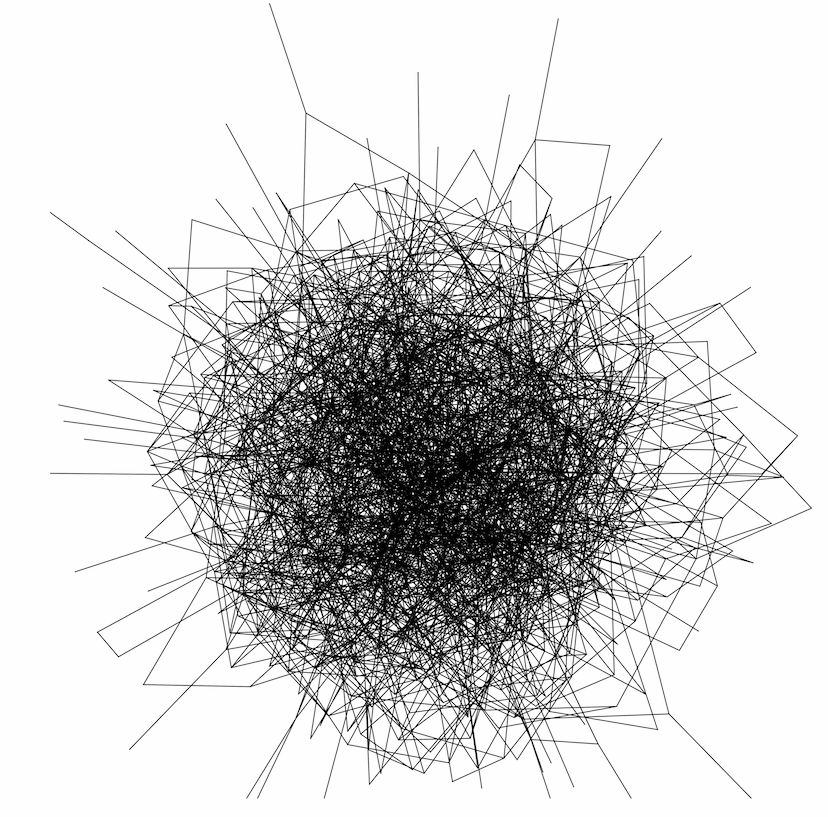
\includegraphics[width=0.45\textwidth,height=0.3\textheight]{figures/random_lowres.png}
\includegraphics[width=0.45\textwidth,height=0.3\textheight]{figures/lattice.png}\\
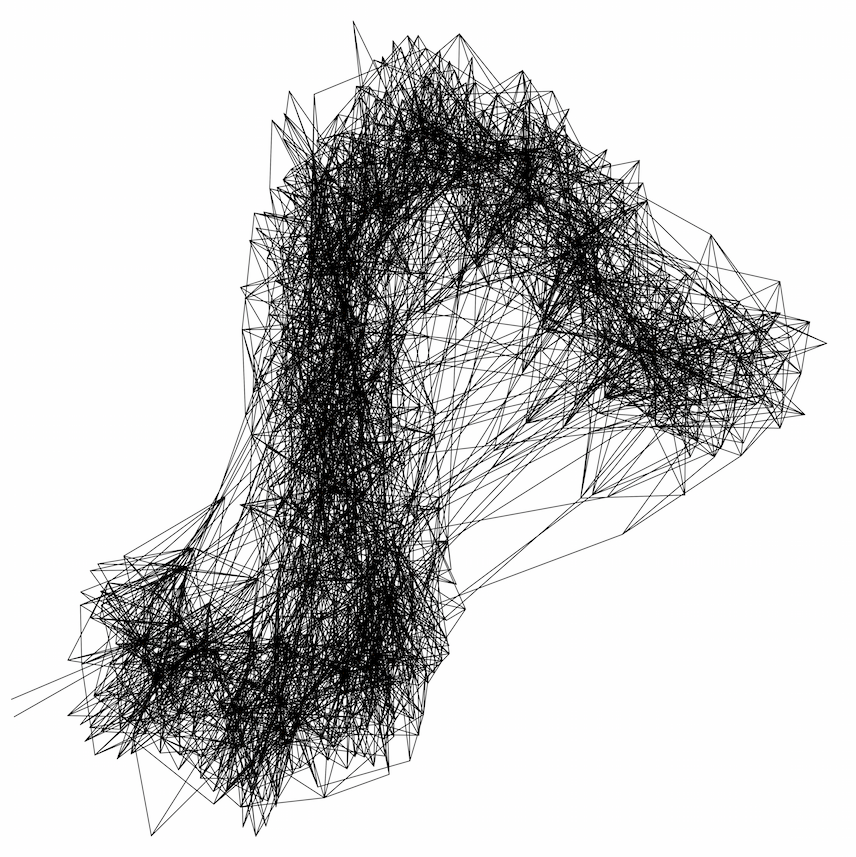
\includegraphics[width=0.45\textwidth,height=0.3\textheight]{figures/pa-age_lowres.png}
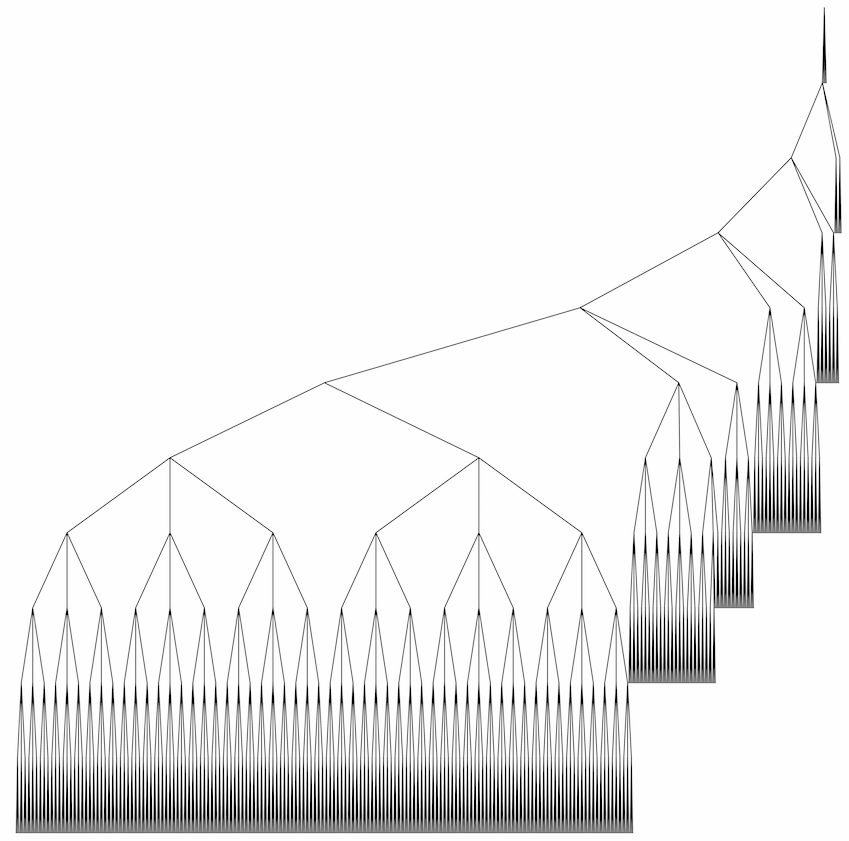
\includegraphics[width=0.45\textwidth,height=0.3\textheight]{figures/tree_lowres.png}
\caption{Représentation d'instances des exemples synthétiques de réseaux. Dans l'ordre de haut en bas et de droite à gauche : réseau aléatoire, grille perturbée, attachement préférentiel, arbre.}
\label{fig:examples}
\end{figure}
%%%%%%%%%%%%%%

%%%%%%%%%%%%%%
\begin{figure}
\centering
\vspace{-1cm}
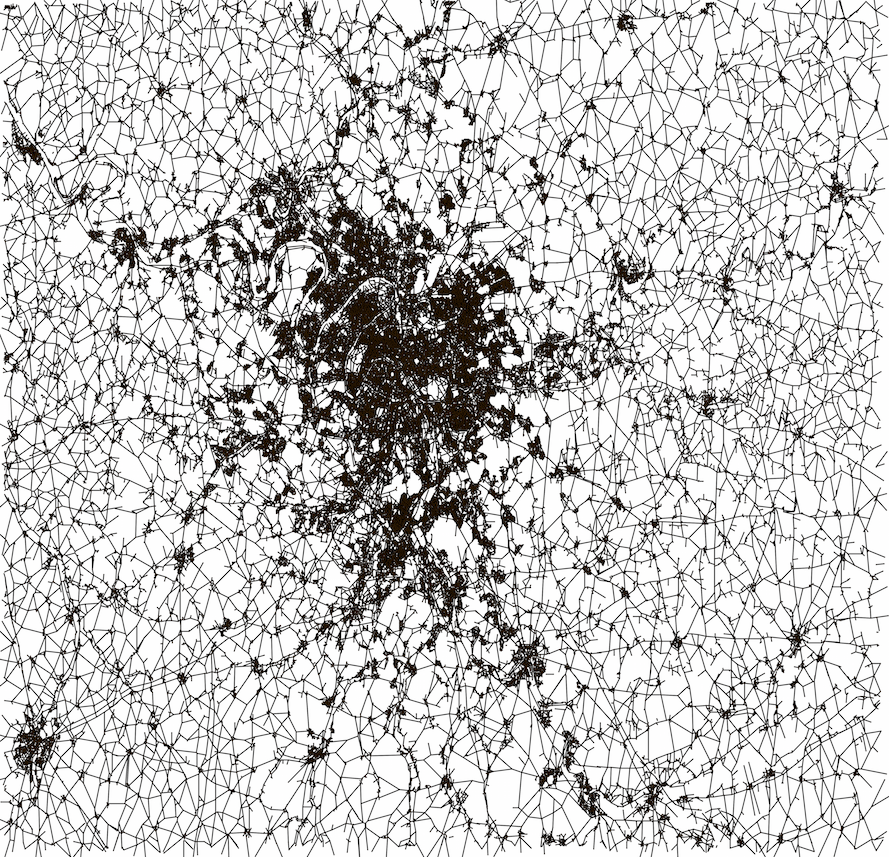
\includegraphics[width=0.45\textwidth,height=0.3\textheight]{figures/idf_lowres.png}
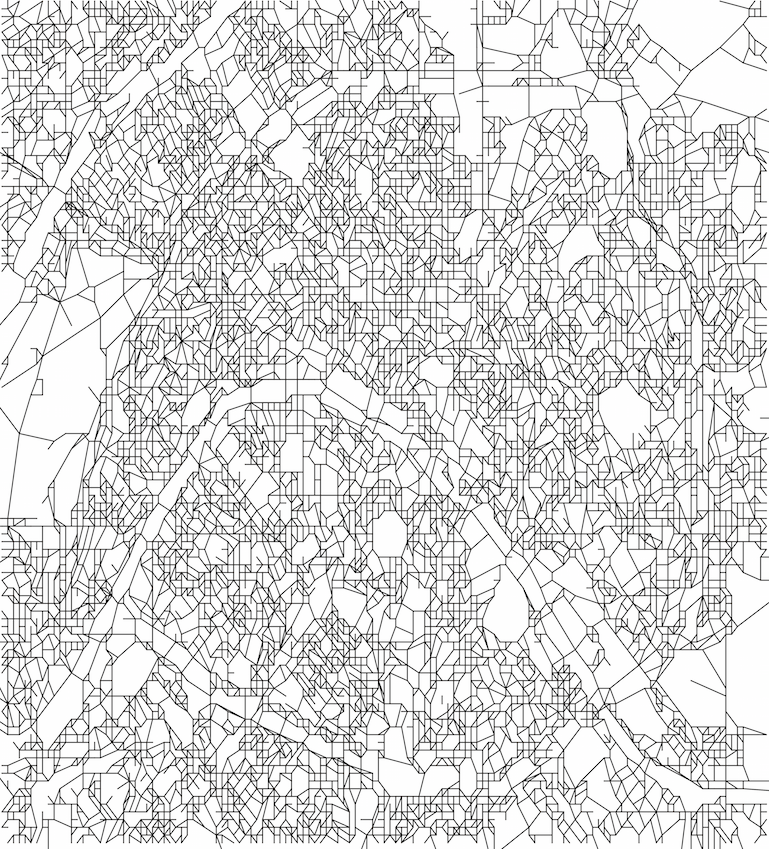
\includegraphics[width=0.45\textwidth,height=0.3\textheight]{figures/paris_lowres.png}\\
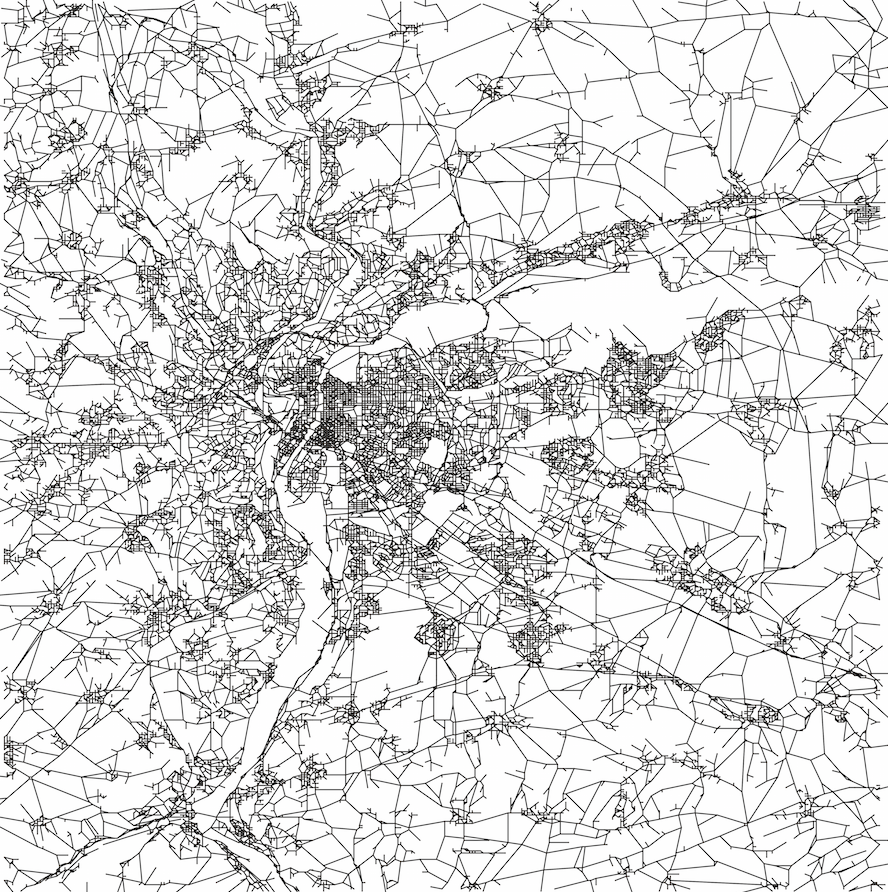
\includegraphics[width=0.45\textwidth,height=0.3\textheight]{figures/lyon_lowres.png}
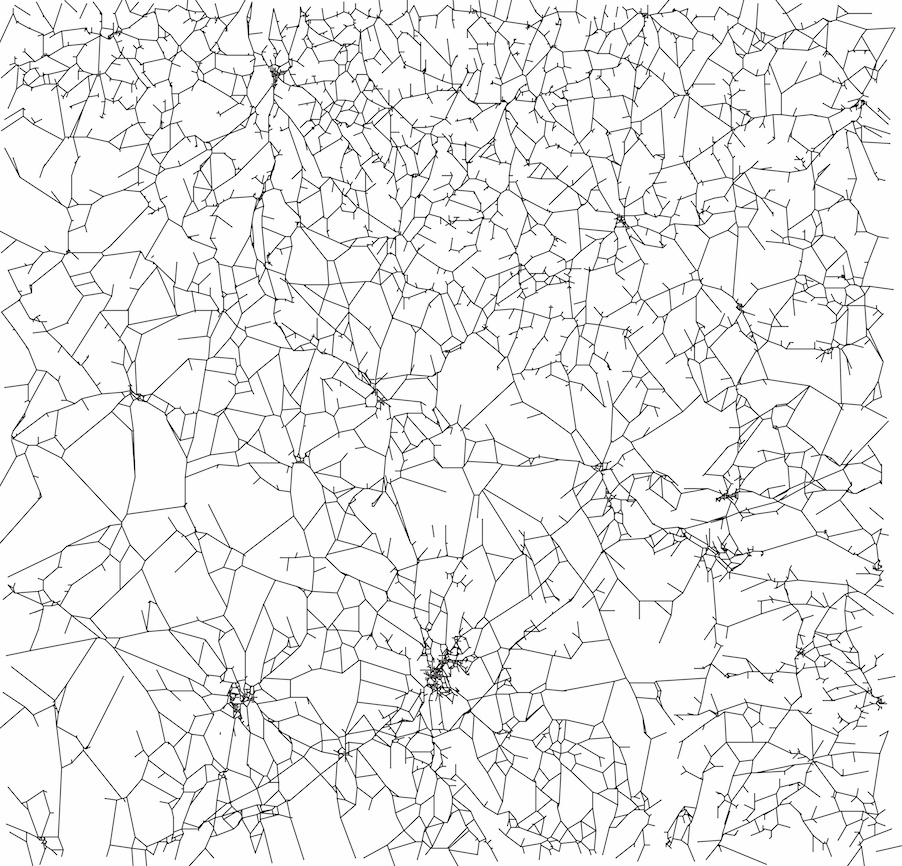
\includegraphics[width=0.45\textwidth,height=0.3\textheight]{figures/lacourtine_lowres.png}\\
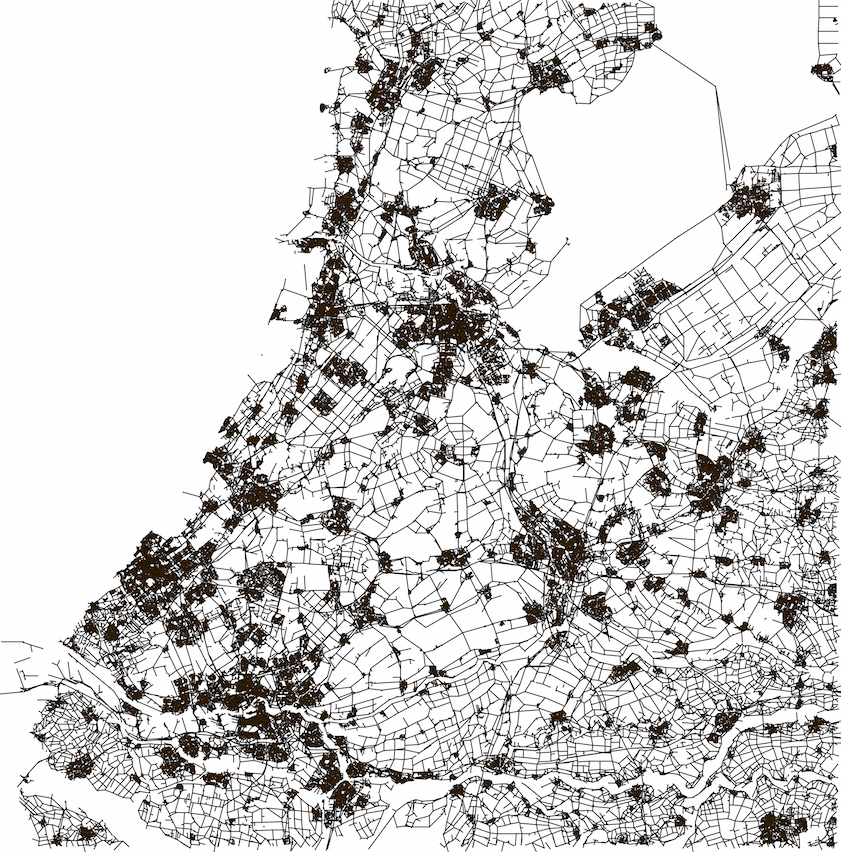
\includegraphics[width=0.45\textwidth,height=0.3\textheight]{figures/randstad_lowres.png}
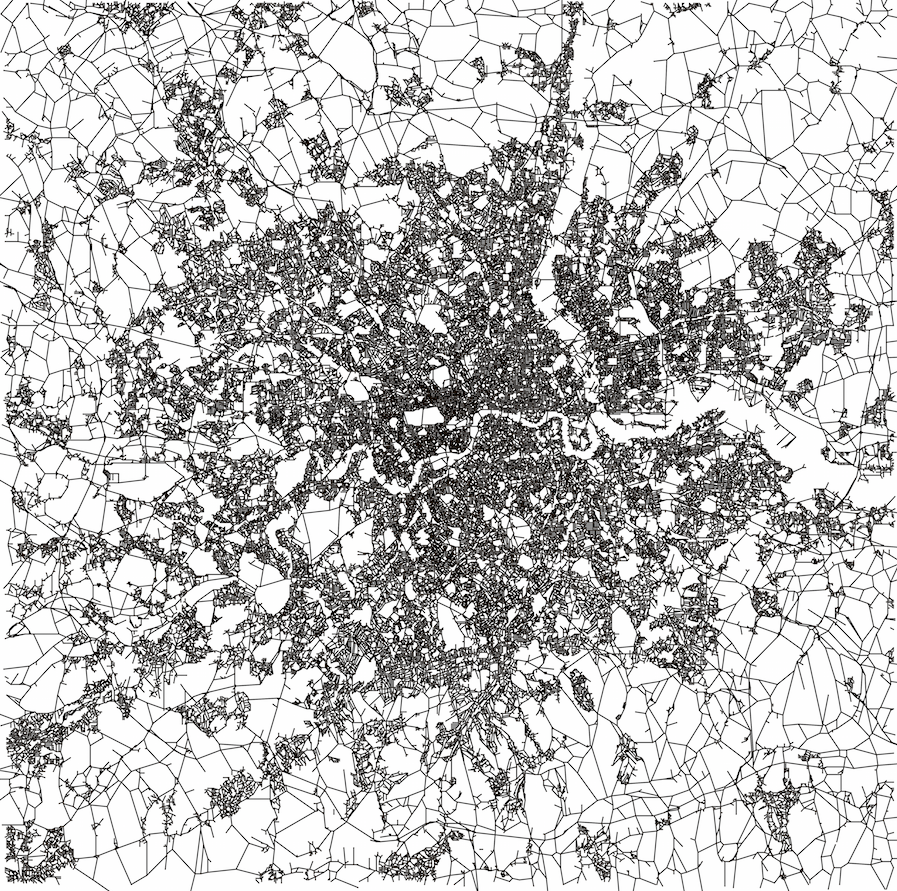
\includegraphics[width=0.45\textwidth,height=0.3\textheight]{figures/londonM25_lowres.png}\\
\caption{Réseaux routiers réels étudiés. Dans l'ordre de haut en bas et de droite à gauche : Ile-de-France, Paris, Grand Lyon, La Courtine, Randstad, London Metropolitan Area}
\label{fig:real}
\end{figure}
%%%%%%%%%%%%%%

%%%%%%%%%%%%%%
\begin{figure}
\centering
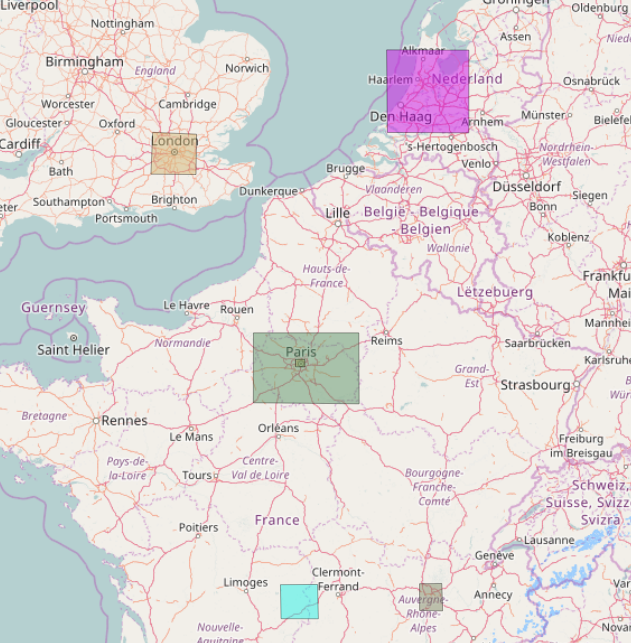
\includegraphics[width=0.8\textwidth]{figures/areas}
\caption{Localisation Géographique des réseaux réels étudiés.}
\label{fig:loc}
\end{figure}
%%%%%%%%%%%%%%


% questions :
% - commentaires sur mesures ?
% - intuitivement, le plus sensible aux perturbations ?
% - matrice des correlations pour chaque type : lecture ; interpretation
% - comment mesurer correlations sur réseaux réels ?
% - vers une mesure dynamique de la résilience : question conceptuelle sur séparation dynamique/topologie - évoquer papier barabasi ?







\strut\hfill$\star$\hspace{1.2cm}$\star$\hfill\strut\vspace{0.1cm}\\

\strut\hfill$\star$\hfill\strut\par








\end{document}